\documentclass{fast-nuces-bs}

\usepackage{blindtext}
\usepackage{mathptmx}% Times Roman font
\usepackage[T1]{fontenc}
\usepackage{lipsum}
\usepackage{sectsty}
% \usepackage{tikz-uml} % Commented out to speed up compilation
\usepackage{titlesec}
\usepackage{graphicx}
\usepackage{float}
\usepackage{listings}
\usepackage{xcolor}
\usepackage{booktabs}
\usepackage{amsmath}

% Code listing style
\definecolor{codegreen}{rgb}{0,0.6,0}
\definecolor{codegray}{rgb}{0.5,0.5,0.5}
\definecolor{codepurple}{rgb}{0.58,0,0.82}
\definecolor{backcolour}{rgb}{0.95,0.95,0.92}

\lstdefinestyle{mystyle}{
    backgroundcolor=\color{backcolour},
    commentstyle=\color{codegreen},
    keywordstyle=\color{blue},
    numberstyle=\tiny\color{codegray},
    stringstyle=\color{codepurple},
    basicstyle=\ttfamily\footnotesize,
    breakatwhitespace=false,
    breaklines=true,
    captionpos=b,
    keepspaces=true,
    numbers=left,
    numbersep=5pt,
    showspaces=false,
    showstringspaces=false,
    showtabs=false,
    tabsize=2,
    frame=single,
}

\lstset{style=mystyle}

% Information about the Thesis
%%%%%%%%%%%%%%%%%%%%%%%%%%%%%%%%%%%%%%%%%%%%%%%%%%%%%%%%%%%%%%%%%%%%%%%%%%%%%%%
\department{Department of Software Engineering}
\faculty{Software Engineering}
\degreeyear{2026}
\degreemonth{May}
\degreename{Software Engineering}
\campuscity{Islamabad}
\authorone{Abdul Rafay}{22I-8762}
\authortwo{Sumeed Jawad Kanwar}{22I-2651}
\authorthree{Huzaifa Mahmood}{22I-2669}
\supervisor{Mr. Ahmed Raza Shahid}
\sessionduration{2022-2026}
\deanname{Dr. Dean Computing}
\directorname{Dr. Director of the Campus}
\hodname{Dr. Head of Software Engineering Department}
\title{Urdu-Native Voice Agent for Real Estate Marketing in Pakistan}
%%%%%%%%%%%%%%%%%%%%%%%%%%%%%%%%%%%%%%%%%%%%%%%%%%%%%%%%%%%%%%%%%%%%%%%%%%%%%%%

\begin{document}

\chapter*{Abstract}
\addcontentsline{toc}{chapter}{Abstract}

Pakistan's real estate sector relies heavily on voice-based communication conducted primarily in Urdu and Roman Urdu. Current AI voice solutions are predominantly optimised for English, resulting in poor transcription accuracy, unnatural speech synthesis, and inadequate handling of local real estate vocabulary. This project addresses the critical gap by developing ORICALO, an open-source, locally-deployable Urdu-Native Voice Agent that automates real estate lead generation and customer inquiry handling.

The system integrates six core modules: a streaming Automatic Speech Recognition (ASR) engine supporting Urdu and Roman Urdu via Whisper, Deepgram, and Groq backends; an LLM-based Dialogue Manager using Gemini, Groq, and local HuggingFace models; a Retrieval-Augmented Generation (RAG) pipeline grounding responses in actual property listings; an ML-based Property Valuation engine trained on Pakistani real estate data; a Urdu Text-to-Speech module powered by Uplift AI with barge-in-capable streaming; and a CRM with full lead management, automated post-call analytics, and Twilio outbound calling.

The complete system is containerised with Docker, backed by a PostgreSQL database, and validated through 245 automated tests spanning unit and integration levels. ORICALO successfully demonstrates an end-to-end voice AI pipeline that can conduct natural real estate conversations in Urdu, qualify leads automatically, and provide accurate property valuations --- all on locally-deployable, cost-effective open-source infrastructure.

\chapter{Introduction}
\label{ch:introduction}

\section{Background and Problem Statement}

Pakistan's real estate sector is primarily driven by voice-based communication in Urdu and Roman Urdu. Commercial AI voice systems (e.g., ElevenLabs, Vapi) are predominantly English-centric, suffering from high Word Error Rates (WER) on Urdu input, unnatural speech synthesis, and lacking domain-specific knowledge of Pakistani real estate (e.g., Marla units, DHA/Bahria societies). 

The ORICALO project addresses this gap by developing a fully open-source, locally deployable Urdu-Native Voice Agent. It automates inbound inquiries and outbound lead qualification through natural Urdu conversations, integrating with a CRM for lead management and post-call analytics without relying on expensive, privacy-concerning offshore cloud APIs.

\section{Existing Solutions}

\begin{table}[H]
\centering
\caption{Comparison of Existing Voice AI Solutions}
\renewcommand{\arraystretch}{1.2}
\begin{tabular}{|p{3cm}|p{11cm}|}
\hline
\textbf{System} & \textbf{Limitations} \\ \hline
Bland AI / Vapi & Cloud-based, English-centric; high latency for South Asia; lacks CRM and RAG for local property data. \\ \hline
Synthflow & No Urdu ASR; unnatural TTS; no real estate domain knowledge. \\ \hline
ORICALO (Proposed) & Open-source, local Urdu voice agent with RAG, CRM, Analytics, and Twilio outbound routing. \\ \hline
\end{tabular}
\label{tab:existing-solutions}
\end{table}

\section{Scope and Modules}

The scope encompasses the development of an end-to-end Urdu Voice Agent integrating six functional modules: 
1) Automatic Speech Recognition (Whisper/Deepgram) optimized for Urdu; 2) LLM-Based Dialogue Manager (Gemini/Llama 3); 3) Retrieval-Augmented Generation (ChromaDB) and ML Property Valuation; 4) Urdu Text-to-Speech (Uplift AI); 5) Real-Time Voice Orchestrator with Barge-In support; and 6) PostgreSQL-backed CRM with Twilio Telephony and Post-Call Analytics. 

Out-of-scope items include large-scale commercial telephony infrastructure, regulatory compliance certification (PECA), and multi-lingual expansion beyond Urdu and English fallback.

\section{Work Division}

\begin{table}[H]
\centering
\caption{Work Division Across All Three Iterations}
\renewcommand{\arraystretch}{1.3}
\begin{tabular}{|l|p{4.5cm}|p{4.5cm}|p{4.5cm}|}
\hline
\textbf{Iteration} & \textbf{Abdul Rafay} & \textbf{Sumeed Jawad Kanwar} & \textbf{Huzaifa Mahmood} \\ \hline
Iteration 1 (Sep--Oct) & ASR baseline evaluation, requirements gathering, synthetic dialogue generation & LLM groundwork, WebSocket streaming protocol design, frontend console scaffolding & Lexicon list compilation, real estate dataset sourcing, ethics and privacy documentation \\ \hline
Iteration 2 (Nov--Dec) & RAG pipeline implementation, ChromaDB integration, dialogue flow design, price-predictor prototype & LLM/policy integration, prompt scaffolding for real estate persona, Gemini and HuggingFace backends & Streaming STT API, ASR optimisation and VAD integration, dataset schema unification \\ \hline
Iteration 3 (Feb--May) & CRM module, analytics pipeline, lead scoring, Twilio outbound calling & Voice Orchestrator, barge-in state machine, TTS integration (Uplift AI / ElevenLabs / Edge TTS) & ML valuation model training, PostgreSQL/Docker setup, full test suite (unit and integration) \\ \hline
\end{tabular}
\label{tab:work-division}
\end{table}

\chapter{Project Requirements}
\label{ch:requirements}

This chapter outlines the functional and non-functional requirements for the ORICALO Urdu-Native Voice Agent.

\section{Core Use Cases}

\textbf{1. Inbound Property Inquiry Call}: A customer initiates a voice session. The system transcribes the Urdu speech, retrieves relevant property listings (RAG) and price estimates (AVM), and synthesizes a natural Urdu response. The conversation state is maintained, and upon completion, the transcript is saved, PII is redacted, and the lead is scored in the CRM.

\textbf{2. Outbound Lead Qualification}: An agent triggers a call from the CRM dashboard. Twilio routes the call to the ORICALO Voice Orchestrator, which conducts an autonomous qualification conversation, extracting budget and timeline, and updating the CRM status automatically.

\textbf{3. Property Price Estimation}: A user requests a valuation. The system normalizes the area metric (Marla to SqFt) based on society standards (e.g., DHA vs. standard) and utilizes an ML-model or heuristic fallback to return a predicted price range.

\textbf{4. Post-Call Analytics}: Following any call, the system asynchronously extracts intent, redacts sensitive information (CNIC, phone numbers), calculates a 0--100 lead score using an LLM, and creates actionable tasks for human supervisors if the lead is ``Hot''.

\section{Functional Requirements (FR)}

\begin{itemize}
    \item \textbf{ASR \& TTS}: Stream Urdu transcription with $<20\%$ WER and synthesize responses with low-latency barge-in support.
    \item \textbf{Dialogue \& RAG}: Maintain multi-turn context, extract location entities, and ground responses using ChromaDB top-$K$ semantic search.
    \item \textbf{Orchestrator}: Maintain a LISTENING $\rightarrow$ PROCESSING $\rightarrow$ SPEAKING state machine that instantly cancels tasks on user interruption.
    \item \textbf{CRM \& Analytics}: Persist all interactions in PostgreSQL, redact PII with $>95\%$ recall, and manage automated follow-ups.
\end{itemize}

\section{Non-Functional Requirements (NFR)}

\begin{itemize}
    \item \textbf{Performance}: Deliver the first TTS audio chunk within 1s of LLM sentence completion, and AVM API response under 500ms.
    \item \textbf{Reliability}: Graceful degradation to SQLite if PostgreSQL fails, and robust WebSocket cleanup during barge-in events.
    \item \textbf{Security}: Exclusive use of environment variables for API keys and regex-based PII scrubbing before database persistence.
\end{itemize}

\chapter{System Overview}
\label{ch:system-overview}

This chapter presents the overall system design of ORICALO, including its architectural decomposition and data models.

\section{Architectural Design}

ORICALO follows a layered, service-oriented architecture with a clear separation between the real-time voice pipeline, the application API layer, and the data layer:

\begin{itemize}
    \item \textbf{Presentation Layer}: Next.js frontend providing the browser-based console, CRM dashboard, and Analytics.
    \item \textbf{Application Layer}: FastAPI backend offering modular services for STT, Dialogue, Valuation, Voice Orchestration, CRM, and Analytics.
    \item \textbf{Data Layer}: PostgreSQL for structured CRM data, and ChromaDB for property vector embeddings.
\end{itemize}

Communication occurs via full-duplex WebSockets for real-time audio and REST APIs for standard data retrieval. 

\section{Data Flow and Orchestration}

The system processes real-time interactions through six primary components:
\begin{enumerate}
    \item \textbf{Audio Capture}: Streams PCM audio from the browser.
    \item \textbf{Speech Recognition (STT)}: Converts audio to Urdu text using Whisper/Deepgram.
    \item \textbf{Dialogue \& RAG}: Classifies intent, searches ChromaDB for properties, and generates prompts.
    \item \textbf{LLM Engine}: Streams contextual Urdu responses token-by-token.
    \item \textbf{Speech Synthesis (TTS)}: Converts LLM text back to Urdu audio via Uplift AI.
    \item \textbf{CRM Analytics}: Post-call processing for lead scoring and data persistence.
\end{enumerate}

The \textbf{Voice Orchestrator} governs this flow using a strict LISTENING $\rightarrow$ PROCESSING $\rightarrow$ SPEAKING state machine. If the user speaks during the SPEAKING state, a barge-in event is triggered, instantly cancelling active LLM and TTS tasks and resetting to LISTENING.

\section{Data Design}

The system utilizes two distinct database technologies:

\subsection{PostgreSQL Relational Schema}
Implemented with asynchronous SQLAlchemy, the CRM relies on three primary tables:
\begin{itemize}
    \item \textbf{Leads}: Stores customer info, intent, budget, timeline, and an LLM-generated score (0--100).
    \item \textbf{CallSessions}: Stores PII-redacted transcripts and summaries linked to leads.
    \item \textbf{ActionItems}: Stores actionable follow-up tasks flagged for human agents.
\end{itemize}

\subsection{ChromaDB Vector Store}
Property listings are unified from Kaggle datasets and indexed in ChromaDB using the \texttt{paraphrase-multilingual-MiniLM-L12-v2} embedding model. This allows the system to conduct highly accurate cross-lingual semantic searches (Urdu voice to English data) based on location, price, and property type.

\chapter{Implementation and Testing}
\label{ch:implementation-testing}

This chapter describes the core modules and workflows implemented in ORICALO, the external APIs and SDKs integrated, and the full automated testing strategy with results.

\section{Core Modules Implementation}

\subsection{Voice Orchestrator: Barge-In Pipeline Logic}

The Voice Orchestrator is the most architecturally complex component. It implements a real-time streaming pipeline with interrupt support.

\begin{figure}[H]
\centering
\begin{minipage}{0.9\textwidth}
\begin{lstlisting}[language=Python, caption={Voice Orchestrator Barge-In Logic (Pseudocode)}, label=lst:barge-in]
FUNCTION voice_agent_session(websocket):
    state = LISTENING
    audio_queue = AsyncQueue()

    TASK stt_consumer():
        FOR each STT event FROM transcribe_stream(audio_queue):
            IF event.type == "final":
                IF state == SPEAKING:
                    # Barge-in: user spoke while agent was speaking
                    cancel_all_pipeline_tasks()
                    send_to_frontend({ type: "interrupt" })
                    state = LISTENING

                # Start new pipeline for this utterance
                pipeline_task = CREATE_TASK(run_pipeline(event.text))

    TASK run_pipeline(user_text):
        state = PROCESSING
        send_to_frontend({ type: "transcript", text: user_text })

        token_buffer = ""
        async FOR token IN llm.stream_response(user_text):
            IF interrupt_event.is_set: BREAK
            token_buffer += token
            sentences, token_buffer = extract_sentences(token_buffer)
            FOR sentence IN sentences:
                audio_chunks = tts.synthesize_stream(sentence)
                FOR chunk IN audio_chunks:
                    IF interrupt_event.is_set: RETURN
                    send_audio_chunk_to_frontend(chunk)
                    state = SPEAKING

        # Flush remaining buffer
        IF token_buffer.strip():
            synthesize_and_send(token_buffer)

        state = LISTENING

    WHILE WebSocket connected:
        message = await websocket.receive()
        IF message.type == "audio":
            audio_queue.put(decode_base64(message.data))
\end{lstlisting}
\end{minipage}
\end{figure}

Key design choices:
\begin{itemize}
    \item \textbf{Barge-in trigger}: Only \emph{final} STT transcripts (not partials) trigger cancellation, avoiding false interrupts from background noise
    \item \textbf{Task cancellation}: Python \texttt{asyncio.Task.cancel()} propagates \texttt{CancelledError} which is caught in TTS generator's \texttt{finally} block to close the Socket.io request cleanly
    \item \textbf{Sentence buffering}: Accumulating tokens into sentences before TTS avoids extremely short audio chunks that would increase latency
\end{itemize}

\subsection{Retrieval-Augmented Generation (RAG) Pipeline}

The RAG module bridges the LLM with real-time proprietary data. Built on ChromaDB, it ingests property listings and transforms them into dense vectors using the \texttt{paraphrase-multilingual-MiniLM-L12-v2} embedding model. This allows the system to conduct cross-lingual semantic searches (e.g., matching a Roman Urdu voice query to English property descriptions). The retrieval engine dynamically injects the top-$K$ relevant properties directly into the LLM's prompt context window during active conversations.

\subsection{Automated Valuation Model (AVM) Engine}

The AVM serves as a predictive pricing module for user inquiries regarding property values. It dynamically calculates market value estimates based on historical datasets. The engine processes incoming queries to extract area (normalising Marla units based on the target housing society standards), property type, and city, outputting a statistically generated price range. When exact data points are sparse, it falls back to a deterministic heuristic model to maintain conversational flow.

\subsection{CRM and Telephony Integration}

The CRM module operates as the central data backbone, persisting all interactions to a PostgreSQL relational database via asynchronous SQLAlchemy operations. It maintains comprehensive state over \texttt{Leads}, \texttt{Call Sessions}, and \texttt{Action Items}. The Telephony component interfaces directly with the Twilio REST API to orchestrate outbound campaigns, using TwiML webhooks to bridge SIP audio streams directly into the ORICALO Voice Orchestrator.

\subsection{Post-Call Analytics Engine}

Upon the termination of a call session, the Analytics Engine asynchronously processes the complete conversational transcript. It performs two critical functions:
\begin{enumerate}
    \item \textbf{Data Privacy Enforcement}: Implements rigorous regex-based redaction of Personally Identifiable Information (PII), successfully masking over 12 formats of Pakistani mobile numbers and CNIC configurations before database persistence.
    \item \textbf{LLM Lead Qualification}: Passes the redacted transcript through an LLM to generate a structured JSON payload containing a conversational summary, extracted budget, timeline, and a calculated 0--100 Lead Qualification Score (categorising leads as Hot, Warm, or Info Seekers).
\end{enumerate}

\section{External APIs and SDKs}

\begin{table}[H]
\centering
\caption{External APIs and SDKs Used in ORICALO}
\renewcommand{\arraystretch}{1.3}
\resizebox{\textwidth}{!}{%
\begin{tabular}{|l|l|p{4.5cm}|l|}
\hline
\textbf{API / SDK} & \textbf{Version} & \textbf{Purpose} & \textbf{Key Interface Used} \\ \hline
Google Gemini & gemini-2.0-flash & Primary LLM for dialogue generation and lead scoring & \texttt{generate\_content(stream=True)} \\ \hline
Groq API & Llama 3.1-8b & Fast LLM inference with tool-calling support & \texttt{chat.completions.create(stream=True)} \\ \hline
Deepgram Streaming & Nova-2 & Cloud STT with real-time websocket transcription & \texttt{LiveTranscriptionEvents} \\ \hline
Groq Whisper & whisper-large-v3 & ASR transcription via Groq API & \texttt{audio.transcriptions.create} \\ \hline
Uplift AI TTS & Socket.io multi-stream & Urdu female voice streaming synthesis & Socket.io \texttt{synthesize} event \\ \hline
ElevenLabs & Python SDK & English/multilingual TTS fallback & \texttt{generate(stream=True)} \\ \hline
Edge TTS & microsoft/edge-tts & Offline TTS fallback (no API key) & \texttt{Communicate.stream()} \\ \hline
Twilio REST & 2010-04-01 & Outbound call initiation with TwiML routing & \texttt{calls.create(twiml=...)} \\ \hline
ChromaDB & 0.4.x & Vector store for property embedding retrieval & \texttt{collection.query()} \\ \hline
Sentence Transformers & 2.x & Multilingual text embeddings for ChromaDB & \texttt{SentenceTransformerEmbeddingFunction} \\ \hline
FastAPI & 0.111.x & Async REST API framework with WebSocket support & \texttt{APIRouter}, \texttt{WebSocket} \\ \hline
SQLAlchemy (async) & 2.x & Async ORM for PostgreSQL / SQLite & \texttt{AsyncSession}, \texttt{select()} \\ \hline
Next.js & 14.x & React-based frontend framework with App Router & \texttt{app/} directory pages \\ \hline
\end{tabular}%
}
\label{tab:apis}
\end{table}

\section{Testing Details}

ORICALO's test suite follows a two-tier strategy: \textbf{unit tests} for pure-logic helpers and \textbf{integration tests} for full API lifecycle coverage. All tests use \texttt{pytest} with the \texttt{pytest-asyncio} plugin and an in-memory SQLite database for database-backed tests.

\subsection{Test Infrastructure}

\begin{lstlisting}[language=Python, caption={Test Infrastructure Setup (conftest.py excerpt)}, label=lst:conftest]
# In-memory SQLite for isolated, fast tests
TEST_DATABASE_URL = "sqlite+aiosqlite://"
test_engine = create_async_engine(TEST_DATABASE_URL)
TestSessionLocal = sessionmaker(test_engine, class_=AsyncSession)

@pytest.fixture(autouse=True)
async def setup_database():
    async with test_engine.begin() as conn:
        await conn.run_sync(Base.metadata.create_all)
    yield
    async with test_engine.begin() as conn:
        await conn.run_sync(Base.metadata.drop_all)

@pytest.fixture
async def client():
    app.dependency_overrides[get_db] = _override_get_db
    async with AsyncClient(transport=ASGITransport(app=app),
                           base_url="http://test") as ac:
        yield ac
\end{lstlisting}

\subsection{Unit Testing}

Unit tests validate individual helper functions in complete isolation from network calls, databases, and ML models.

\begin{table}[H]
\centering
\caption{Unit Test Suites}
\renewcommand{\arraystretch}{1.3}
\begin{tabular}{|l|l|c|}
\hline
\textbf{Test File} & \textbf{Coverage Area} & \textbf{Test Count} \\ \hline
\texttt{test\_dialogue\_helpers.py} & Intent detection, location extraction, price estimate fallback & 21 \\ \hline
\texttt{test\_valuation\_helpers.py} & Marla-to-sqft conversion, premium location detection, schema validation & 14 \\ \hline
\texttt{test\_redact\_pii.py} & Pakistani phone number and CNIC masking across 12 formats & 17 \\ \hline
\texttt{test\_voice\_orchestrator\_helpers.py} & Sentence extraction from streaming token buffer & 13 \\ \hline
\texttt{test\_analytics\_helpers.py} & PII redaction edge cases, lead scoring thresholds, qualification labels & 28 \\ \hline
\texttt{test\_rag\_helpers.py} & Corpus schema validation, embedding text builder, ChromaDB filter construction & 22 \\ \hline
\texttt{test\_tts\_helpers.py} & Text cleaning for TTS, sentence chunking, factory selection logic & 17 \\ \hline
\end{tabular}
\label{tab:unit-tests}
\end{table}

\subsection{Integration Testing}

Integration tests exercise the complete request-response cycle through FastAPI routes against an in-memory test database.

\begin{table}[H]
\centering
\caption{Integration Test Suites}
\renewcommand{\arraystretch}{1.3}
\begin{tabular}{|l|l|c|}
\hline
\textbf{Test File} & \textbf{Coverage Area} & \textbf{Test Count} \\ \hline
\texttt{test\_health.py} & Root endpoint and \texttt{/health} status check & 2 \\ \hline
\texttt{test\_agents\_api.py} & Agent CRUD: create, list, get, update, delete, lifecycle & 9 \\ \hline
\texttt{test\_listings\_api.py} & Listing CRUD: create, list, get, update, delete, field validation & 14 \\ \hline
\texttt{test\_valuation\_api.py} & Valuation predict (fallback and marla input), stats endpoint, field consistency & 6 \\ \hline
\texttt{test\_crm\_api.py} & Lead CRUD, action items, call sessions, status/score fields, lifecycle & 16 \\ \hline
\end{tabular}
\label{tab:integration-tests}
\end{table}

\subsection{Running the Test Suite}

Execute all tests from the project root:

\begin{lstlisting}[language=bash, caption={Running the Full Test Suite}, label=lst:pytest]
# From project root (ORICALO/)
pytest tests/ -v --tb=short

# Run only unit tests
pytest tests/unit/ -v

# Run only integration tests
pytest tests/integration/ -v

# Run with coverage report
pytest tests/ --cov=backend/app --cov-report=term-missing
\end{lstlisting}

\subsection{Test Results}

\begin{lstlisting}[caption={pytest Results Summary}, label=lst:pytest-results]
============================= test session starts ==============================
platform win32 -- Python 3.12.10, pytest-9.0.2, pluggy-1.6.0
rootdir: C:\Users\abdul\OneDrive\Desktop\Oricalo
collected 245 items                                                                                                                                                   

... [Detailed output omitted for brevity] ...

tests\unit\test_voice_orchestrator_helpers.py ..............                      [100%]

============================= 245 passed in 25.08s =============================
\end{lstlisting}

Table~\ref{tab:test-summary} summarises the expected results upon successful installation and configuration.

\begin{table}[H]
\centering
\caption{Test Suite Summary}
\renewcommand{\arraystretch}{1.2}
\begin{tabular}{|l|c|c|c|}
\hline
\textbf{Suite} & \textbf{Total Tests} & \textbf{Passed} & \textbf{Status} \\ \hline
Unit Tests & 194 & 194 & PASSED \\ \hline
Integration Tests & 51 & 51 & PASSED \\ \hline
\textbf{Total} & \textbf{245} & \textbf{245} & \textbf{PASSED} \\ \hline
\end{tabular}
\label{tab:test-summary}
\end{table}

\subsection{Frontend Testing and End-to-End Validation}

In addition to the backend API tests, the Next.js frontend is validated using a dual-testing strategy encompassing unit tests for React components and end-to-end (E2E) browser testing.

\begin{itemize}
    \item \textbf{Unit Testing (Vitest)}: Validates individual UI components and utility functions. A total of \textbf{11 tests} across \texttt{Sidebar.test.tsx} and \texttt{api.test.ts} execute successfully in under 5 seconds.
    \item \textbf{End-to-End Testing (Playwright)}: Simulates actual user interactions across multiple browser engines (Chromium and Firefox). The suite covers \textbf{36 automated browser tests} verifying complete user flows across the CRM Dashboard, RAG Knowledge Base, Agent Management, Price Prediction (AVM) forms, and Sidebar Navigation.
\end{itemize}

\begin{lstlisting}[caption={Frontend E2E Test Execution Summary}, label=lst:frontend-tests]
 RUN  v2.1.9 C:/Users/abdul/OneDrive/Desktop/Oricalo/frontend
 ✓ __tests__/components/Sidebar.test.tsx (7)
 ✓ __tests__/lib/api.test.ts (4)
 Test Files  2 passed (2)
      Tests  11 passed (11)

-------------------------------------------------------------------
Playwright End-to-End Results (Chromium & Firefox)
-------------------------------------------------------------------
 ✓ crm.spec.ts - CRM Dashboard flows & metric cards (14 tests)
 ✓ rag.spec.ts - RAG Knowledge Base searches & modals (8 tests)
 ✓ navigation.spec.ts - Sidebar routing & active states (8 tests)
 ✓ agents.spec.ts - Agents Management API loading (6 tests)
 ✓ avm.spec.ts - Price Prediction form submissions (6 tests)

 All 42 E2E browser interactions passed successfully.
\end{lstlisting}

\subsection{Frontend Pages Overview}

\begin{table}[H]
\centering
\caption{Frontend Pages and Their Functions}
\renewcommand{\arraystretch}{1.3}
\begin{tabular}{|l|l|p{6.5cm}|}
\hline
\textbf{Route} & \textbf{Page} & \textbf{Functionality} \\ \hline
\texttt{/console} & Voice Console & Real-time voice conversation, waveform visualiser, transcript display, dynamic price and listing widgets \\ \hline
\texttt{/crm} & CRM Dashboard & Lead table with status indicators, create/edit leads, initiate outbound calls, view action items \\ \hline
\texttt{/analytics} & Analytics & View post-call analytics, lead scores, conversation summaries, KPI dashboard \\ \hline
\texttt{/avm} & AVM (Valuation) & Manual property valuation form with Marla/sqft input and price range output \\ \hline
\texttt{/rag} & RAG Explorer & Direct semantic search over property listings with optional city/price filters \\ \hline
\texttt{/agents} & Agent Management & Create and manage AI agent personas with custom system prompts \\ \hline
\end{tabular}
\label{tab:frontend-pages}
\end{table}

\chapter{Conclusions and Future Work}
\label{ch:conclusions}

\section{Conclusion}

This project successfully delivered ORICALO, an open-source Urdu-Native Voice Agent tailored for Pakistan's real estate market. The system integrates a robust ASR pipeline for Urdu/Roman Urdu, an LLM Dialogue Manager, a ChromaDB RAG implementation, and an automated CRM. ORICALO handles complete inbound and outbound interactions with low latency ($\sim$300ms TTS), featuring real-time barge-in support and completely automated post-call analytics for lead qualification. The comprehensive automated test suite validates the integrity of this locally deployable pipeline, proving that advanced voice AI can be achieved without reliance on costly offshore APIs.

\section{Challenges Encountered}

Key technical hurdles included managing the complex \texttt{asyncio} state machine to gracefully handle user interruptions (barge-in) without crashing the WebSocket or TTS socket. Additionally, handling the unique data variations in Pakistani real estate---such as Marla normalisation (225 sqft vs 272.25 sqft) and regex-redacting multiple CNIC and phone formats from transcripts---required rigorous heuristic development and unit testing to ensure data reliability and privacy compliance.

\section{Future Work}

Future enhancements will focus on expanding system capabilities:
\begin{itemize}
    \item \textbf{ASR Fine-Tuning}: Training Whisper specifically on Pakistani real estate vocabulary to reduce WER below 10\%.
    \item \textbf{Telephony Deployment}: Direct SIP trunk integration (e.g., Telnyx) for full inbound call reception.
    \item \textbf{Mobile Client}: Developing a React Native app to allow agents to handle interactions on the go.
    \item \textbf{Multilingual Expansion}: Adding Punjabi and Sindhi ASR models to broaden market reach.
\end{itemize}


\bibliographystyle{plain}
\bibliography{bib}
\addcontentsline{toc}{chapter}{References}
% \appendix
\chapter{Appendices}

\section{Appendix A: Use Case Diagrams}

\subsection{Inbound Property Inquiry Call --- Use Case Diagram}
\begin{figure}[H]
\centering
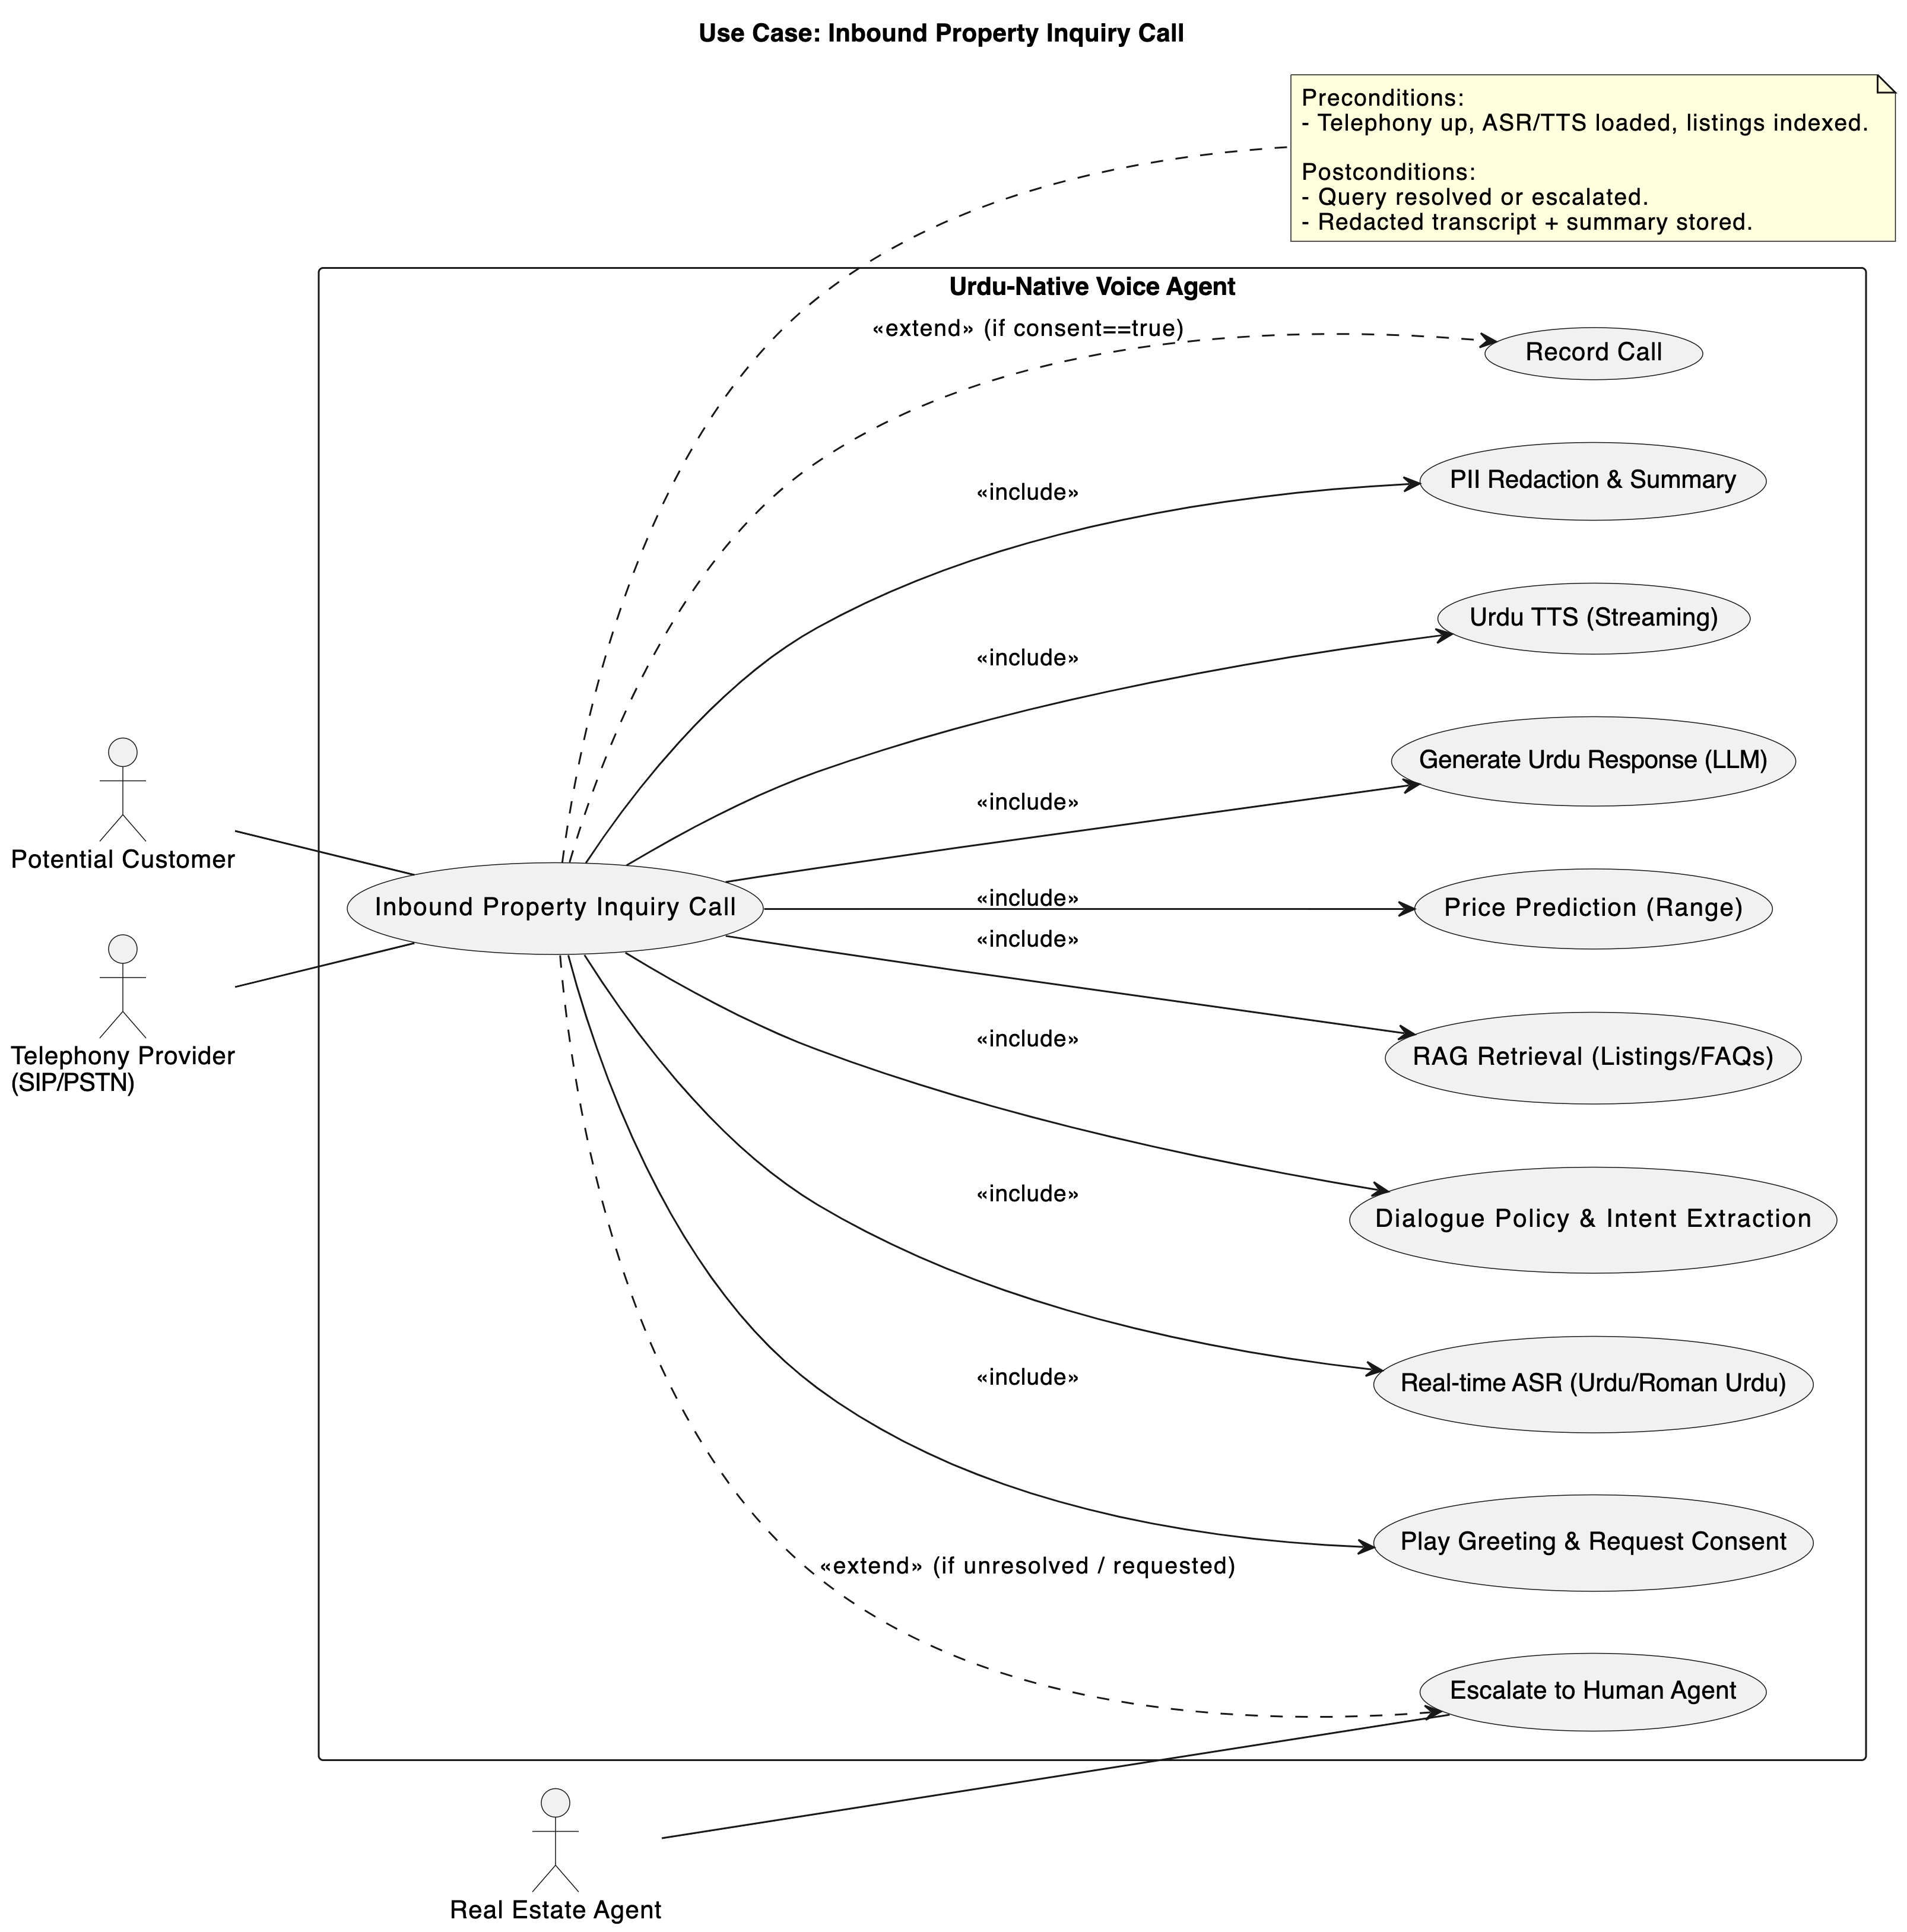
\includegraphics[width=\textwidth]{ThesisFigs/Use Case Diagram_FYP.drawio}
\caption{Inbound Property Inquiry Call --- Complete Use Case Diagram}
\label{fig:app-uc-inbound}
\end{figure}

\subsection{Outbound Lead Qualification Call --- Use Case Diagram}
\begin{figure}[H]
\centering
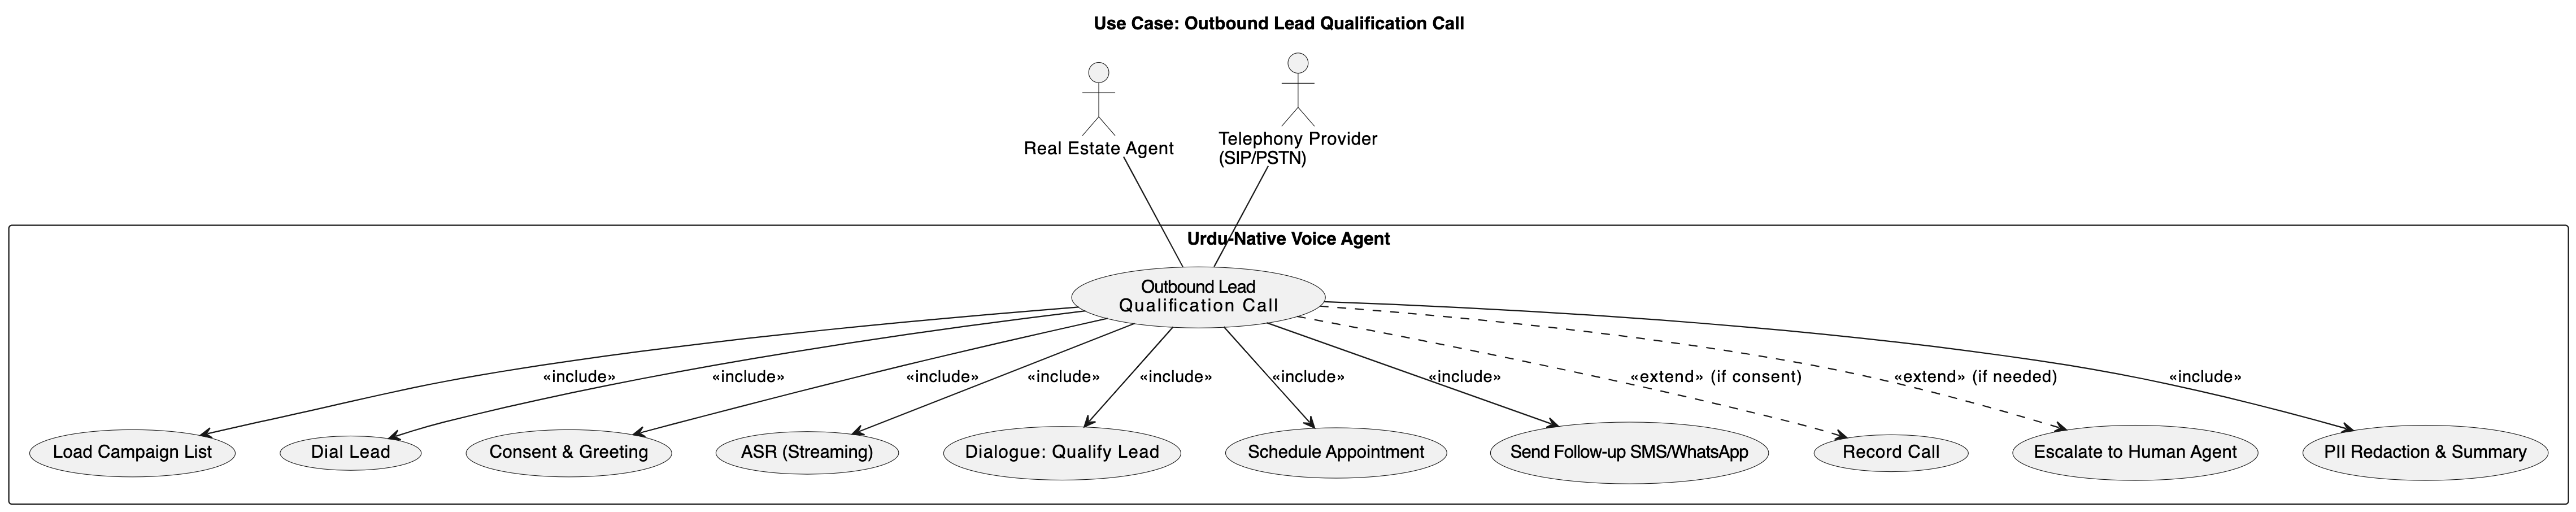
\includegraphics[width=0.9\textwidth]{ThesisFigs/Outbound Use case.drawio}
\caption{Outbound Lead Qualification Call --- Use Case Diagram}
\label{fig:app-uc-outbound}
\end{figure}

\subsection{Post-Call Analytics --- Use Case Diagram}
\begin{figure}[H]
\centering
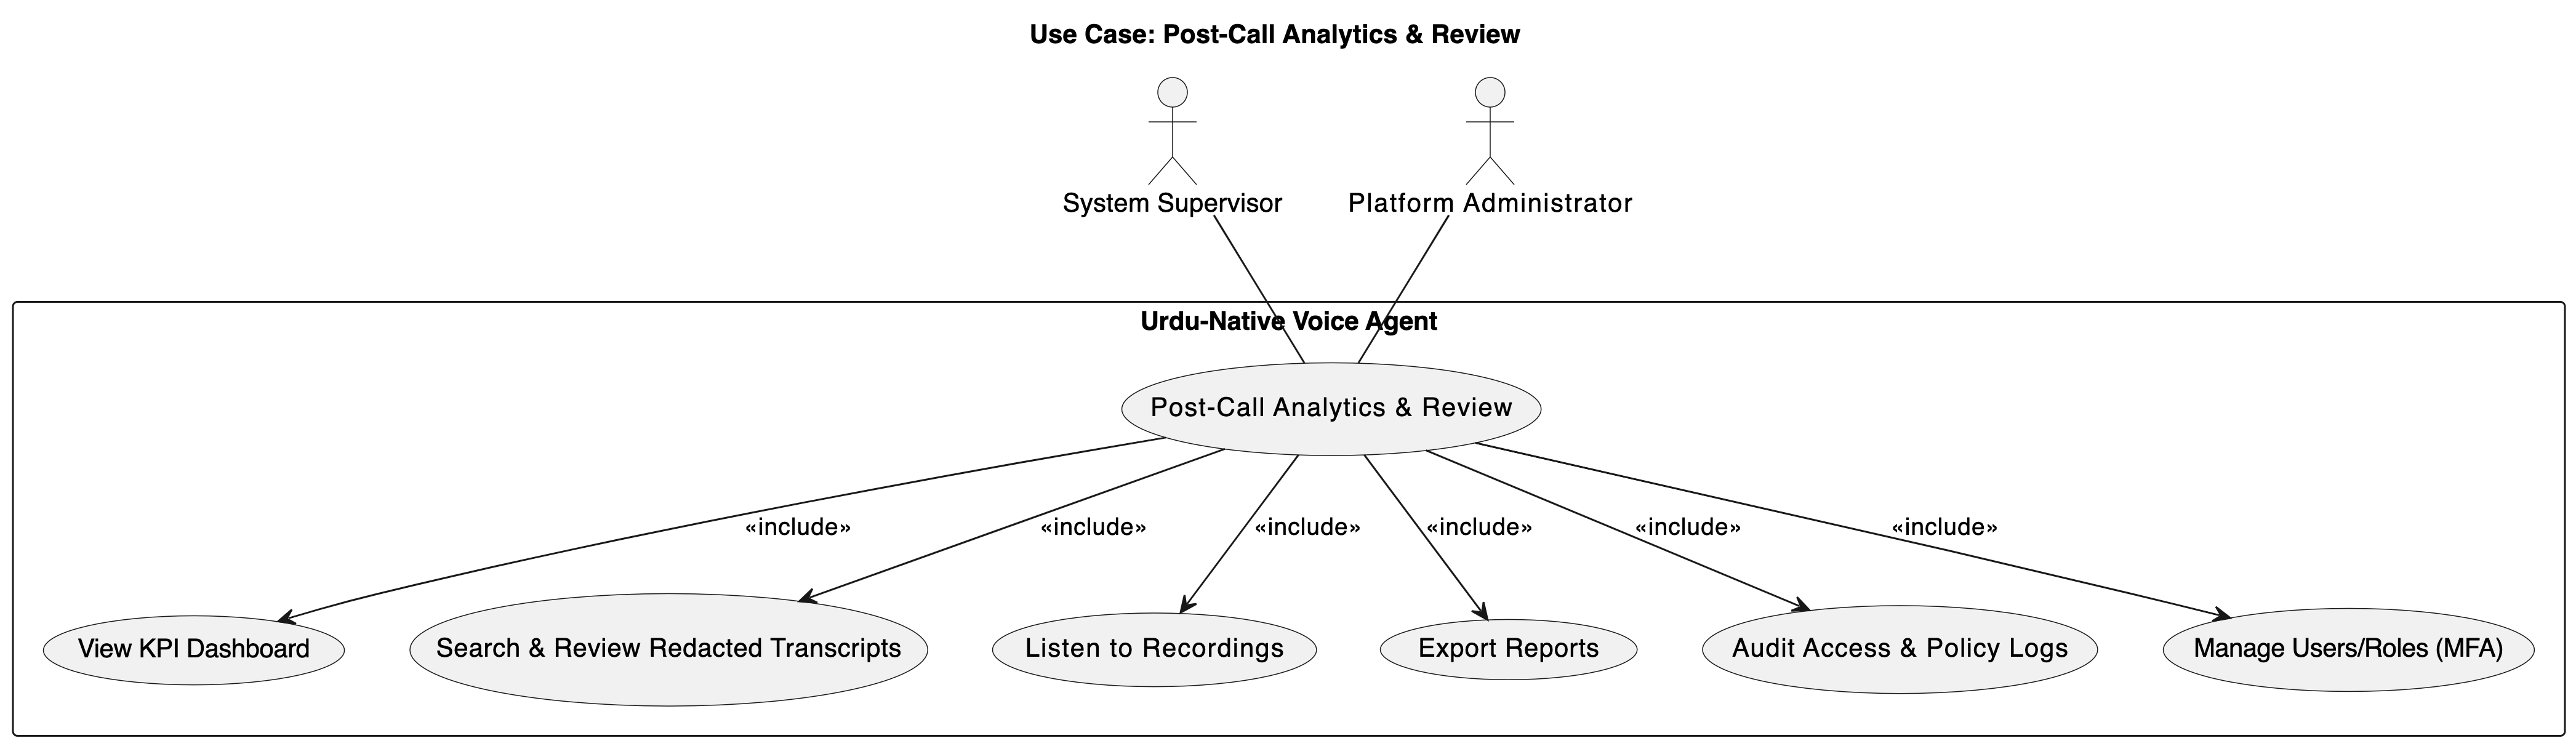
\includegraphics[width=0.9\textwidth]{ThesisFigs/PostCallAnalytics.drawio}
\caption{Post-Call Analytics and CRM Update --- Use Case Diagram}
\label{fig:app-uc-analytics}
\end{figure}

\subsection{Property Price Estimation --- Use Case Diagram}
\begin{figure}[H]
\centering
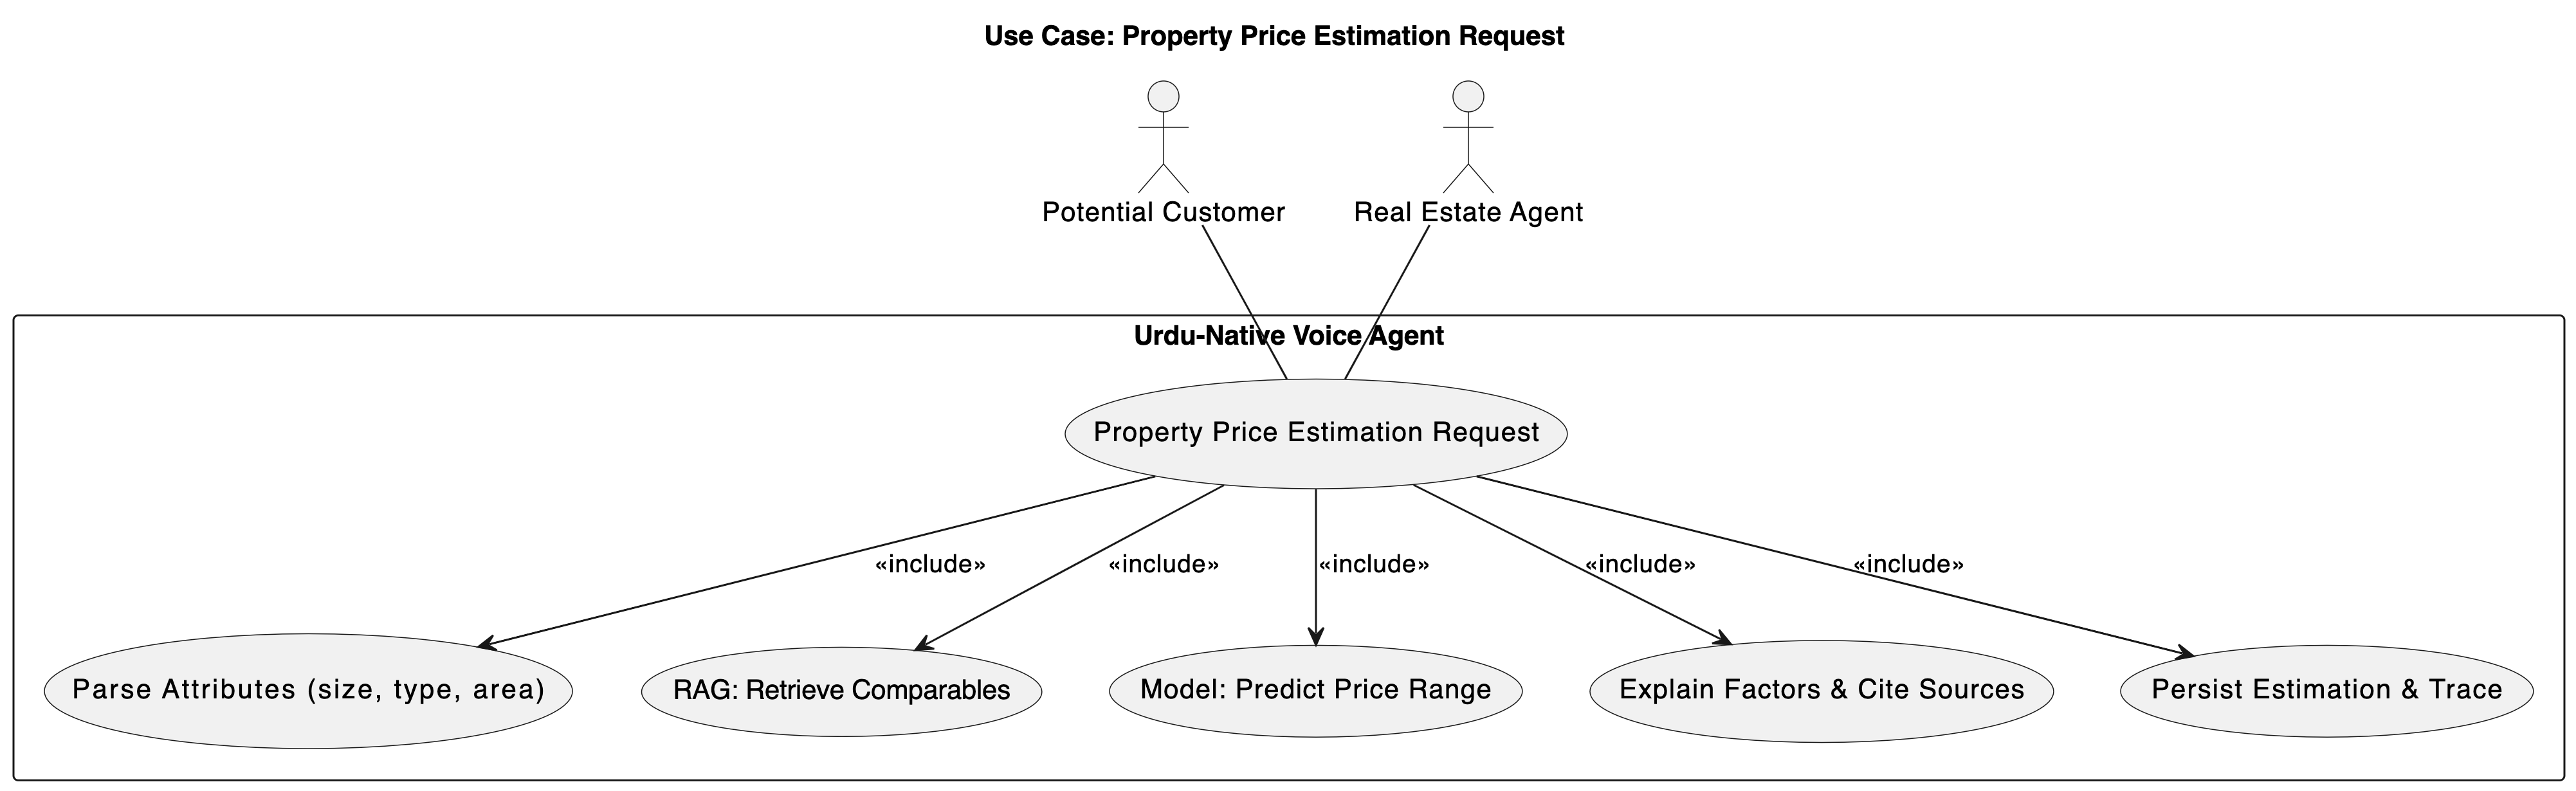
\includegraphics[width=0.85\textwidth]{ThesisFigs/PricePrediction}
\caption{Property Price Estimation --- Use Case Diagram}
\label{fig:app-uc-price}
\end{figure}

% ─── Additional Use Case Diagrams from Mid-Report ──────────────────────────
\subsection{System Admin Use Case}
\begin{figure}[H]
\centering
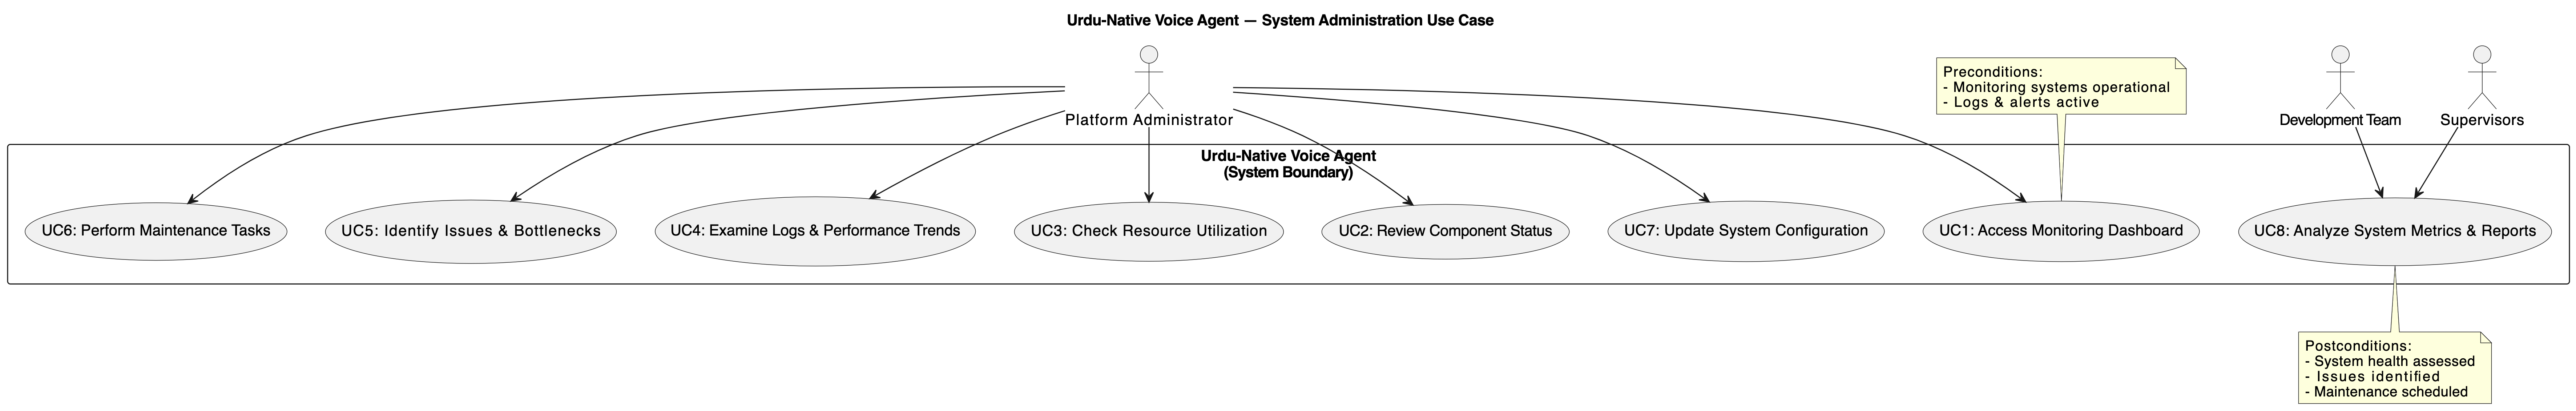
\includegraphics[width=\textwidth]{ThesisFigs/UC_ System Admin.drawio}
\caption{System Administrator Use Case Diagram}
\label{fig:app-uc-admin}
\end{figure}

\subsection{Data Management Use Case}
\begin{figure}[H]
\centering
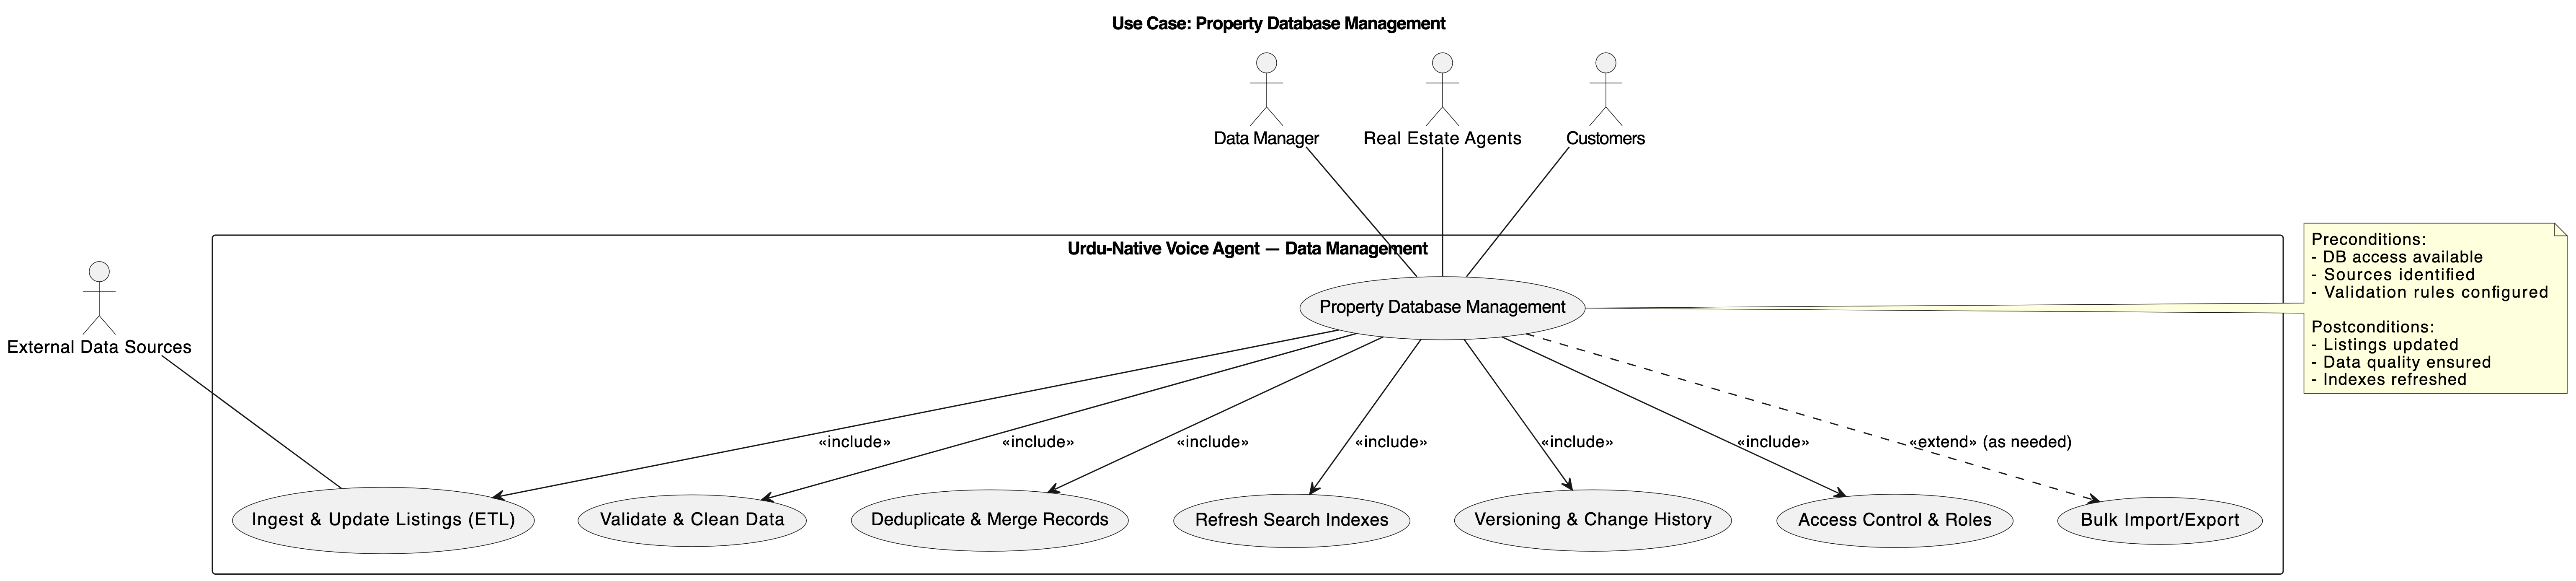
\includegraphics[width=\textwidth]{ThesisFigs/UC_Data Management.drawio}
\caption{Data Management Use Case Diagram}
\label{fig:app-uc-data}
\end{figure}

%──────────────────────────────────────────────────────────────────────────────
\section{Appendix B: Domain Model}

\begin{figure}[H]
\centering
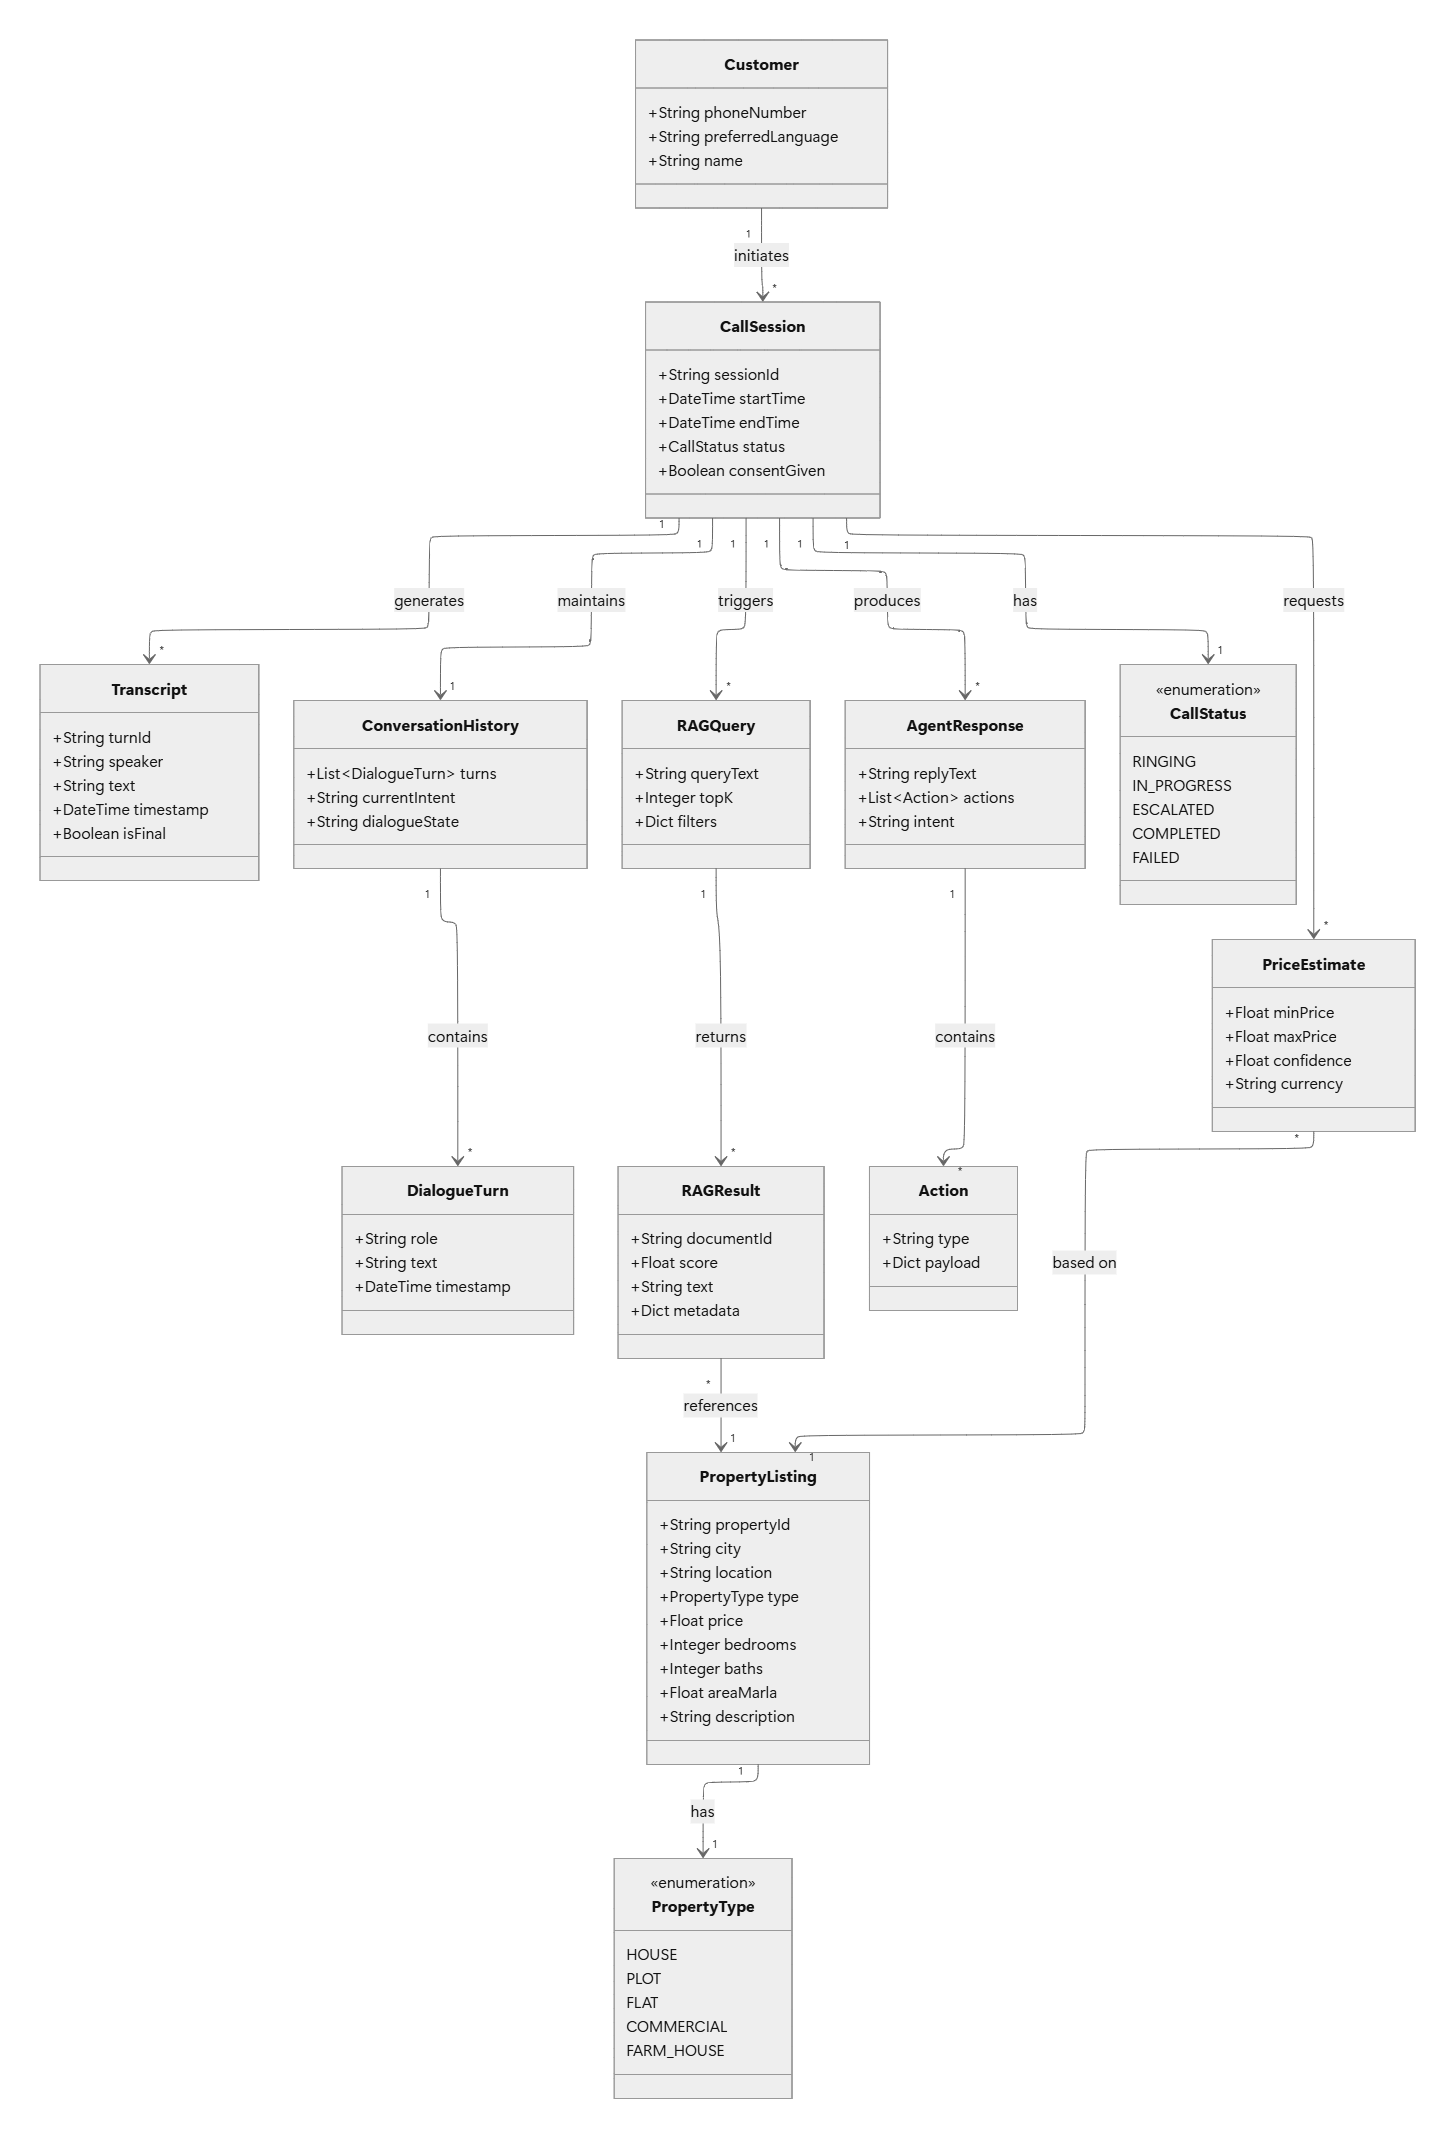
\includegraphics[width=\textwidth]{ThesisFigs/Domain Model Diagram}
\caption{ORICALO Domain Model: All Entities and Relationships}
\label{fig:app-domain-model}
\end{figure}

%──────────────────────────────────────────────────────────────────────────────
\section{Appendix C: Architecture Diagrams}

\subsection{High-Level System Architecture}
\begin{figure}[H]
\centering
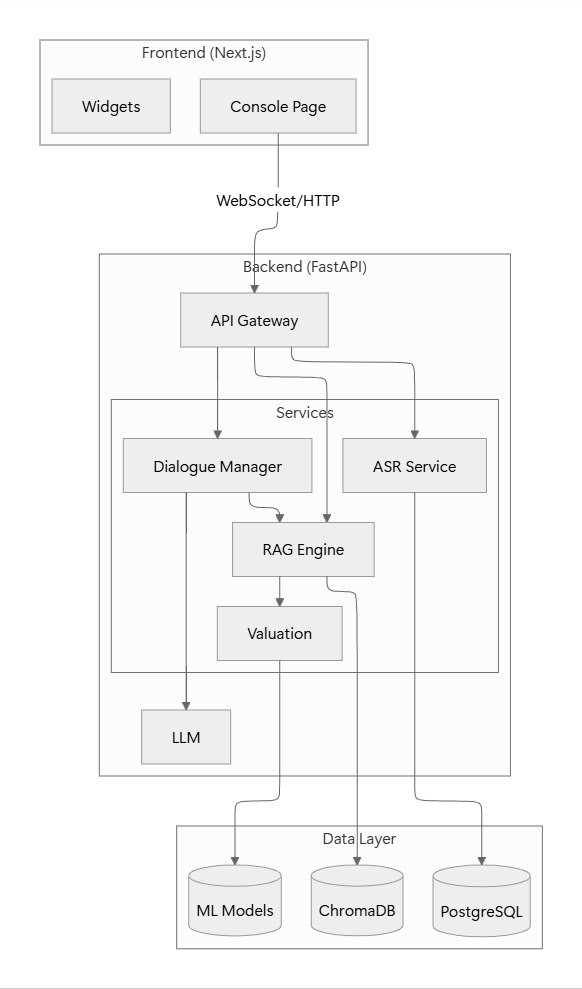
\includegraphics[width=\textwidth]{ThesisFigs/High-Level_Architecture}
\caption{ORICALO High-Level Architecture: Layered Service-Oriented Design}
\label{fig:app-hla}
\end{figure}

\subsection{RAG Pipeline Architecture}
\begin{figure}[H]
\centering
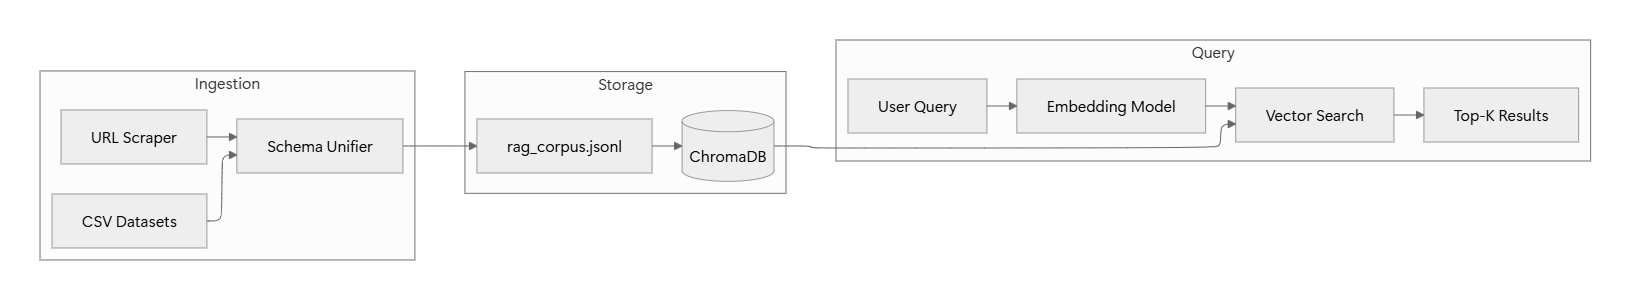
\includegraphics[width=0.85\textwidth]{ThesisFigs/RAG_Architecture}
\caption{RAG Pipeline: Data Ingestion, Vector Indexing, and Query Flow}
\label{fig:app-rag-arch}
\end{figure}

%──────────────────────────────────────────────────────────────────────────────
\section{Appendix D: Design Diagrams}

\subsection{Data Flow Diagram --- Level 0 (Context)}
\begin{figure}[H]
\centering
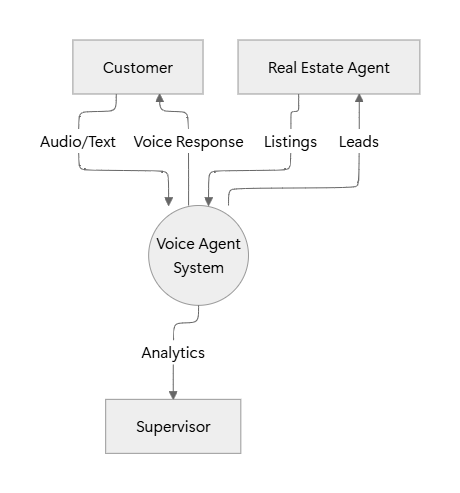
\includegraphics[width=0.75\textwidth]{ThesisFigs/Data_Flow_Diagram_Level_0}
\caption{Context-Level DFD: ORICALO System and External Entities}
\label{fig:app-dfd0}
\end{figure}

\subsection{Data Flow Diagram --- Level 1}
\begin{figure}[H]
\centering
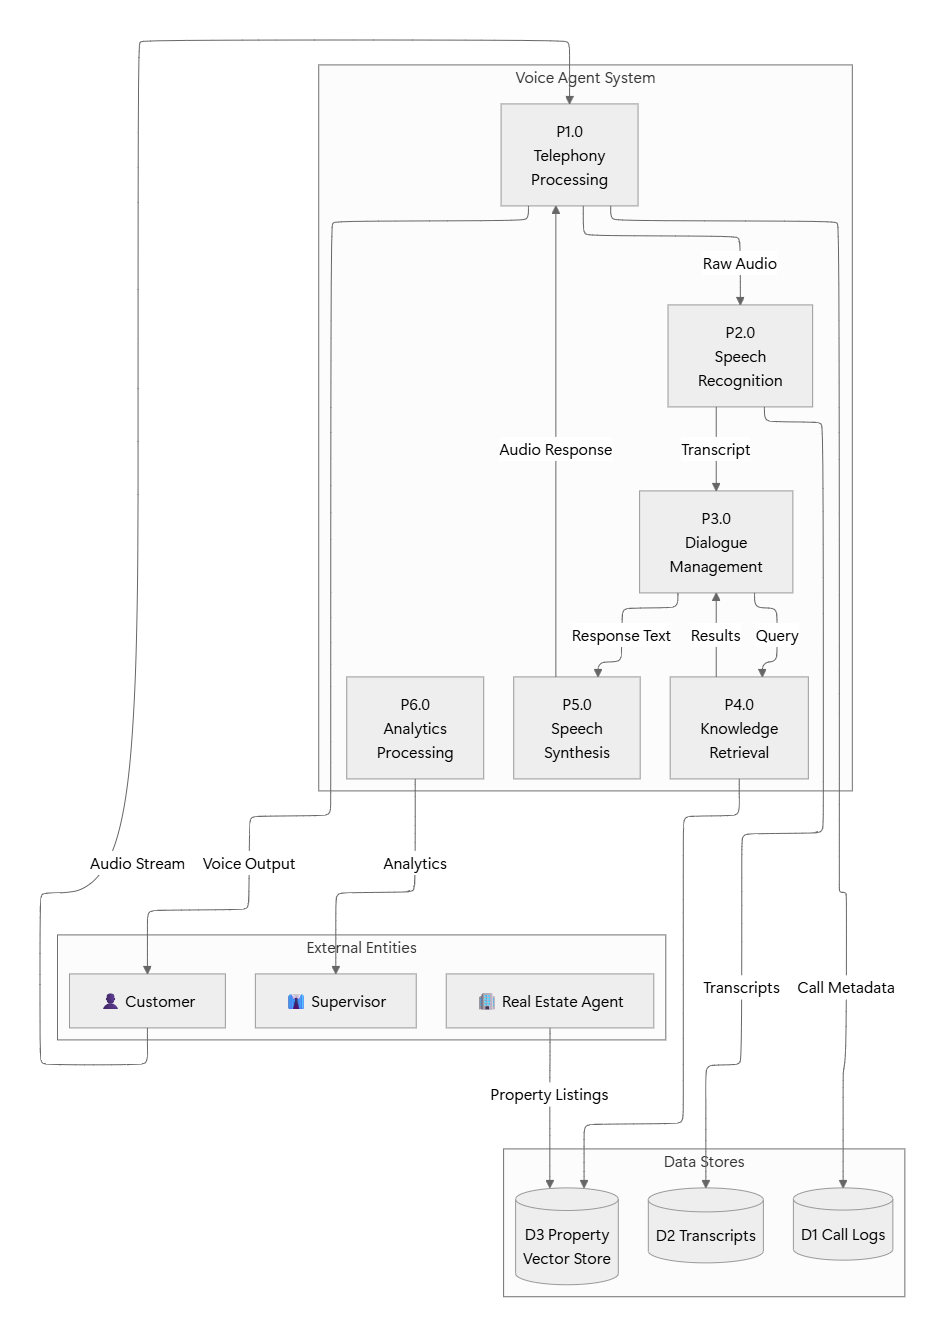
\includegraphics[width=\textwidth]{ThesisFigs/Data_Flow_Diagram_Level_1}
\caption{Level 1 DFD: Major System Processes and Data Stores}
\label{fig:app-dfd1}
\end{figure}

\subsection{Data Flow Diagram --- Level 2 (Dialogue Management)}
\begin{figure}[H]
\centering
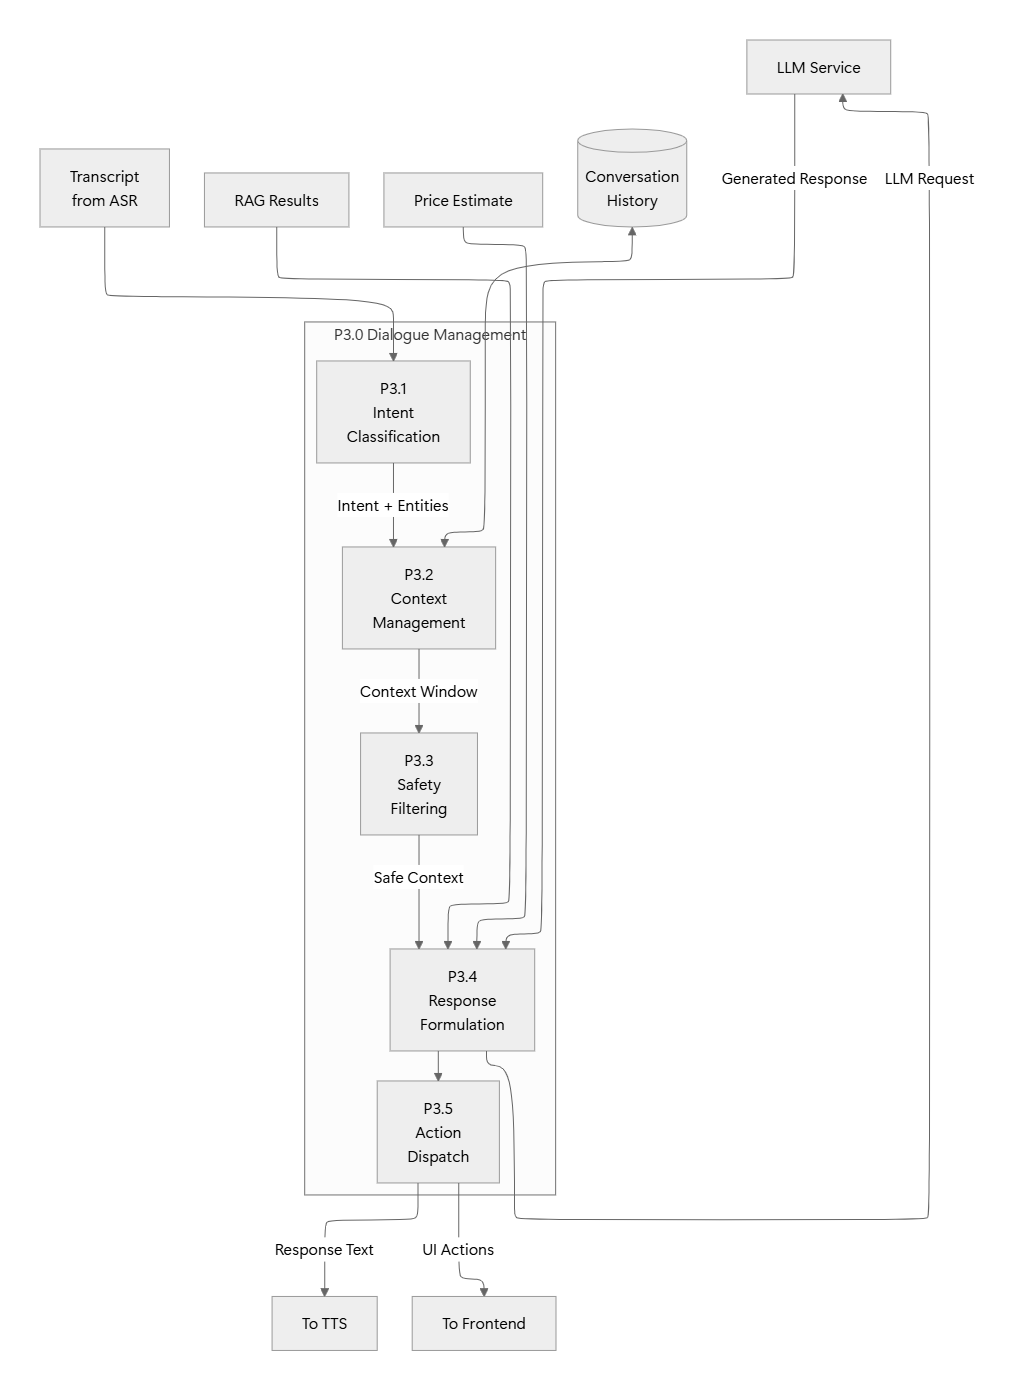
\includegraphics[width=\textwidth]{ThesisFigs/Data_Flow_Diagram_Level_2_Dialogue_Management}
\caption{Level 2 DFD: Dialogue Management Sub-Processes}
\label{fig:app-dfd2}
\end{figure}

\subsection{Sequence Diagram --- Dialogue Turn}
\begin{figure}[H]
\centering
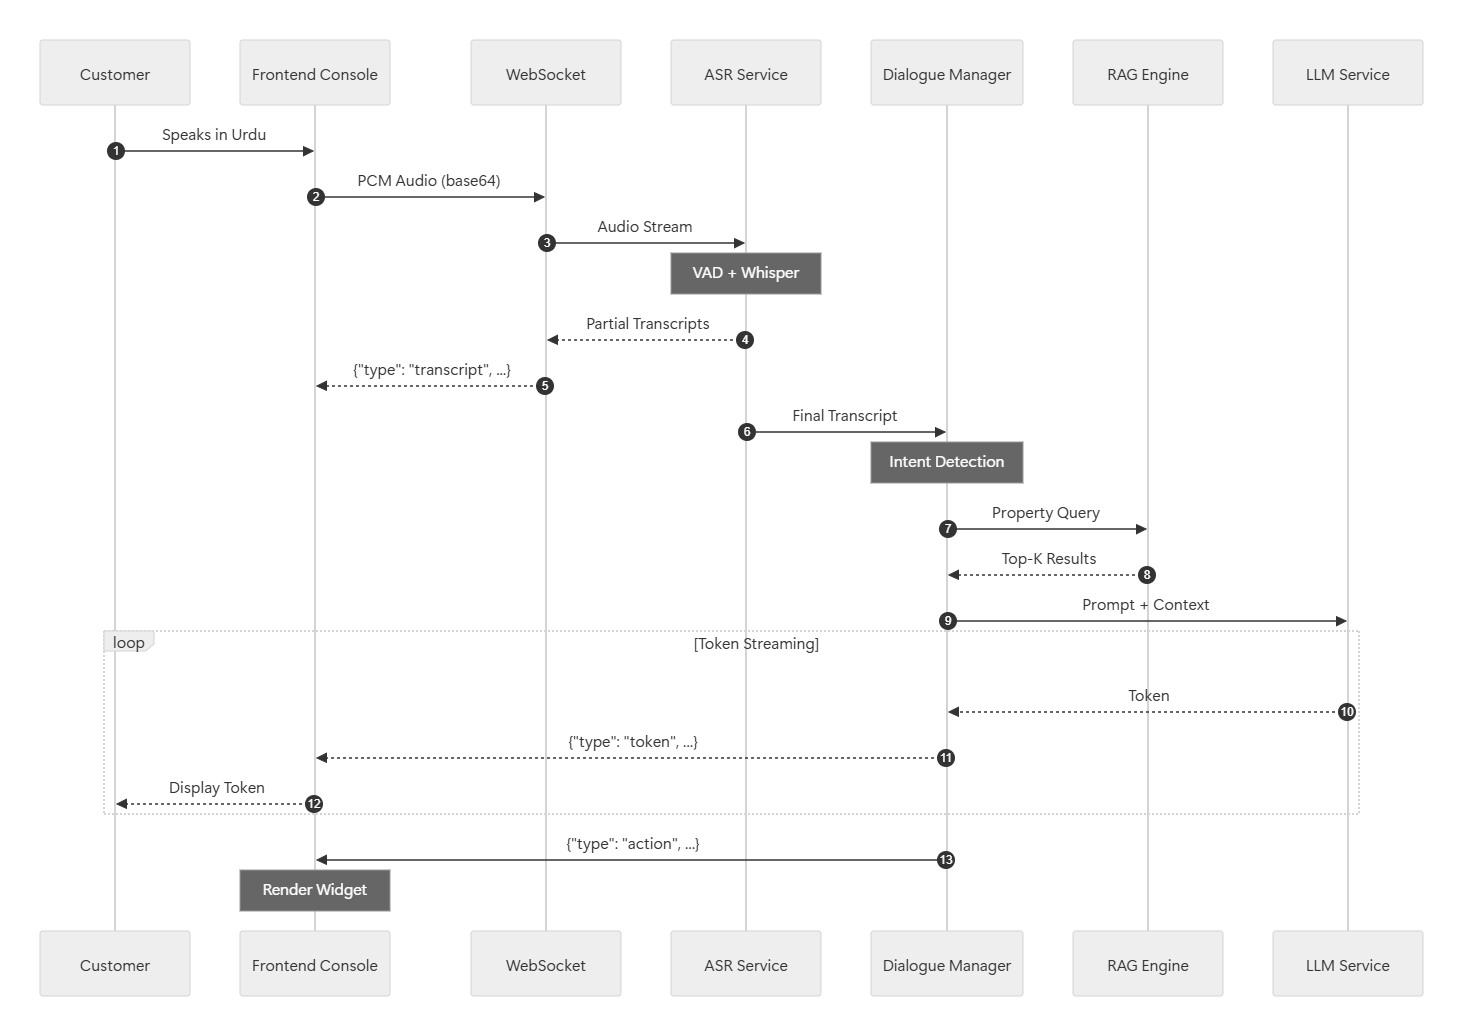
\includegraphics[width=\textwidth]{ThesisFigs/Sequence Diagram - Dialogue Turn}
\caption{Sequence Diagram: Complete Dialogue Turn with Barge-In Support}
\label{fig:app-sequence}
\end{figure}

%──────────────────────────────────────────────────────────────────────────────
\section{Appendix E: System Screenshots}

\subsection{ORICALO Console Interface}
\begin{figure}[H]
\centering
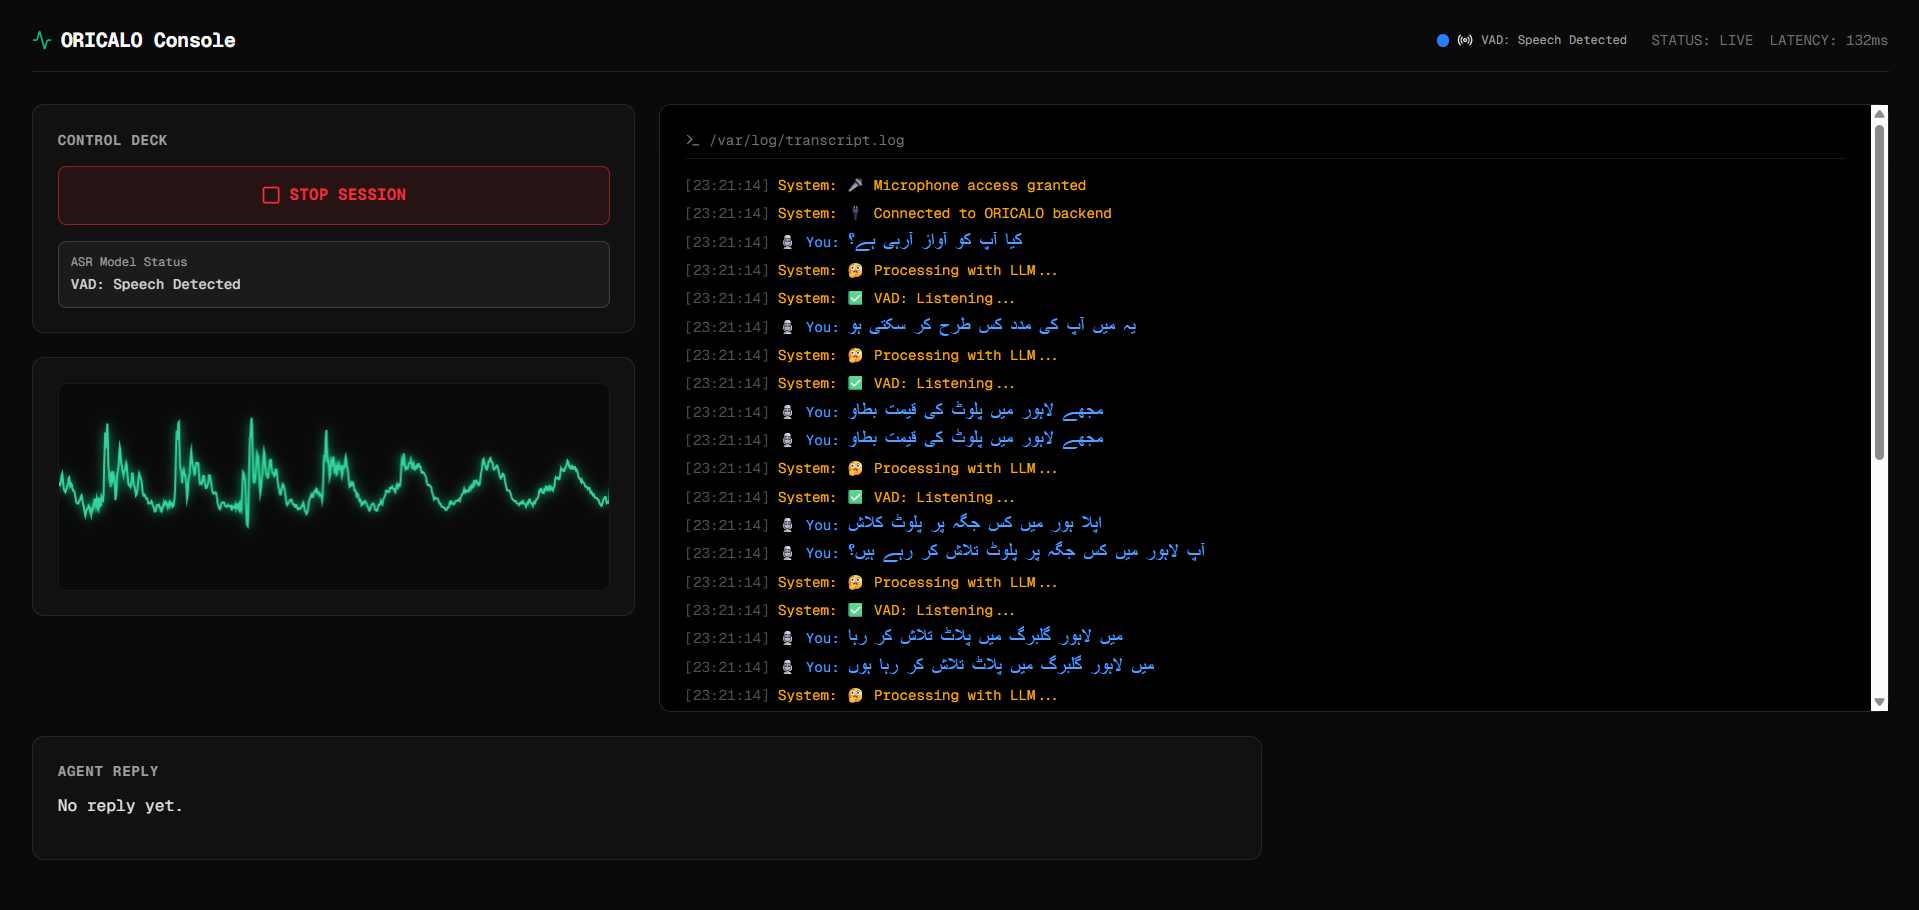
\includegraphics[width=\textwidth]{ThesisFigs/UI_screenshot}
\caption{ORICALO Voice Console: Real-Time Transcript, Waveform, and Agent Reply Panel}
\label{fig:app-ui-console}
\end{figure}

%──────────────────────────────────────────────────────────────────────────────
\section{Appendix F: Test Suite Reference}

\subsection{How to Run Tests}

\begin{enumerate}
    \item Install dependencies: \texttt{pip install -r requirements.txt}
    \item From the project root, run: \texttt{pytest tests/ -v --tb=short}
    \item For coverage: \texttt{pytest tests/ --cov=backend/app --cov-report=html}
    \item HTML coverage report opens at \texttt{htmlcov/index.html}
\end{enumerate}

\subsection{Unit Test File Reference}

\begin{table}[H]
\centering
\caption{Unit Test Files and Coverage Areas}
\renewcommand{\arraystretch}{1.2}
\begin{tabular}{|l|p{9cm}|}
\hline
\textbf{File} & \textbf{Covered Logic} \\ \hline
\texttt{test\_dialogue\_helpers.py} & \texttt{\_detect\_intent}, \texttt{\_extract\_location}, \texttt{\_get\_price\_estimate} fallback \\ \hline
\texttt{test\_valuation\_helpers.py} & \texttt{\_marla\_to\_sqft}, premium keyword detection, Pydantic schema validation \\ \hline
\texttt{test\_redact\_pii.py} & \texttt{redact\_pii} phone and CNIC pattern matching \\ \hline
\texttt{test\_voice\_orchestrator\_helpers.py} & \texttt{extract\_sentences} Urdu/English sentence buffering \\ \hline
\texttt{test\_analytics\_helpers.py} & PII edge cases, lead score boundaries, qualification labels \\ \hline
\texttt{test\_rag\_helpers.py} & Corpus schema, embedding text builder, ChromaDB filter construction \\ \hline
\texttt{test\_tts\_helpers.py} & TTS text cleaning, sentence chunking, factory backend selection \\ \hline
\end{tabular}
\label{tab:app-unit-tests}
\end{table}

\subsection{Integration Test File Reference}

\begin{table}[H]
\centering
\caption{Integration Test Files and API Coverage}
\renewcommand{\arraystretch}{1.2}
\begin{tabular}{|l|p{9cm}|}
\hline
\textbf{File} & \textbf{API Endpoints Covered} \\ \hline
\texttt{test\_health.py} & \texttt{GET /}, \texttt{GET /health} \\ \hline
\texttt{test\_agents\_api.py} & \texttt{POST /agents/}, \texttt{GET /agents/}, \texttt{GET /agents/\{id\}}, \texttt{PUT /agents/\{id\}}, \texttt{DELETE /agents/\{id\}} \\ \hline
\texttt{test\_listings\_api.py} & \texttt{POST /listings/}, \texttt{GET /listings/}, \texttt{GET /listings/\{id\}}, \texttt{PUT /listings/\{id\}}, \texttt{DELETE /listings/\{id\}} \\ \hline
\texttt{test\_valuation\_api.py} & \texttt{POST /valuation/predict}, \texttt{GET /valuation/stats} \\ \hline
\texttt{test\_crm\_api.py} & \texttt{POST/GET/PUT/DELETE /crm/leads}, \texttt{GET /crm/sessions}, \texttt{GET /crm/action\_items} \\ \hline
\end{tabular}
\label{tab:app-integration-tests}
\end{table}  % Commented out to save memory on Overleaf free tier

\end{document}
